\section{Electrophysiological Measurement Distributions from Experimental Literature}\label{sec:data-sources}
Organized, publicly available electrophysiological measurements from single, biological neurons can form an optimization target.
Together, they can be used to parameterize the suite of tests against which a model is optimized.
Optimization makes corresponding model electrophysiological measurements as similar as possible to those observed in biological neurons.

\subsection{NeuroElectro}
One general source of such measurements is The NeuroElectro Project \citep{tripathy2014neuroelectro}, which contains experimental values for 47 distinct electrophysiological measurements across 235 different neuron types.
As with most of the data discussed here, most (but not all) of these measurements were obtained from slice physiology experiments in rodents.
These measurements were programatically extracted from peer-reviewed journal articles over a $\sim20$ year period from $\sim1990-2012$,
and are made easy to access by an application programming interface (API) that NeuronUnit provides bindings to.
Importantly, the measured values--even for a single neuron type--reflect experiments done in many labs using (in some cases) variable methods.
Therefore, the mean of these values (e.g. the mean input resistance across reported Purkinje cells) averages over heterogeneity across cells within a slice, slices within an animal, animals within a lab, and labs within the field.
The sample size for one measure (e.g. input resistance) may be larger than for another (e.g. resting potential) meaning that they may reflect different subsets of experiments.
With those caveats in mind, NeuroElectro is still the most direct way to get a large number of optimization-constraining data values for most neuron types.

In order to verify that the data from NeuroElectro was plausible and was being captured correctly for the purposes of the work in this thesis, I used the API along with a batch visualization pipeline to  visualize the distributions of electrophysiological measurements and inspect them for a) quality control and b) evidence of multimodality.
Multimodality, meaning multiple peaks in the histogram of a single measurement type for a single cell, could be evidence of a physiological heterogeneity not easily explained by random measurement error.
Two peaks in the histogram, for example, could result from two distinct subclasses of a single nominal neuron type, each with its own (narrower) distribution of the same measurement.
In some instances, the mean and standard deviation alone well-described the measurement distributions, as would be expected for random, normally-distributed measurements of a single cell type under reasonably consistent conditions.
These values were then ``approved" for use in model-fitting.
In other cases, these conditions were not met, as exemplified in the figures below.

%\begin{comment}
%\begin{figure}
%\centering
%   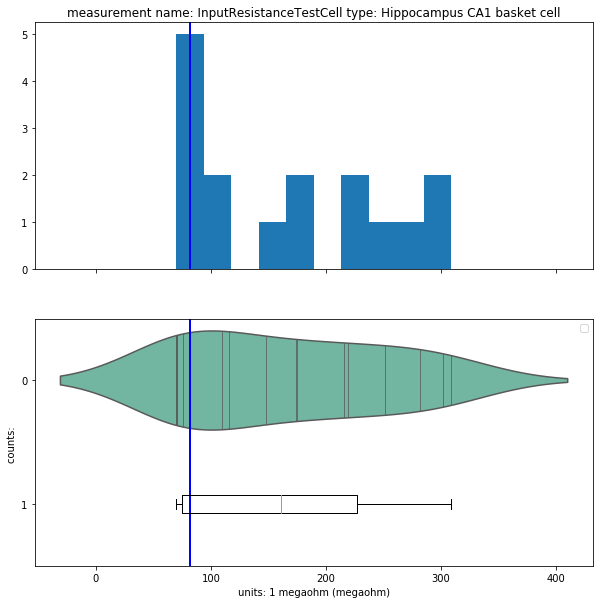
\includegraphics[scale=0.8]{notebooks_converted/needata_thesis_files/needata_thesis_5_5}
%\end{figure}

%\caption{Model parameterization of the brian2 simulator with the customization: interpolated spike height, forced to be above $0mV$}
%
%  \label{fig:sub1}
%\end{subfigure}%
%\begin{figure}
%\centering
%  \includegraphics[scale=0.8]{notebooks_converted/needata_thesis_files/needata_thesis_5_6}
%\end{figure}

%    
%    %\caption{Default model parameterization of the custom written integrator}
%  \label{fig:sub2}
%
%\begin{subfigure}
%  \centering
%      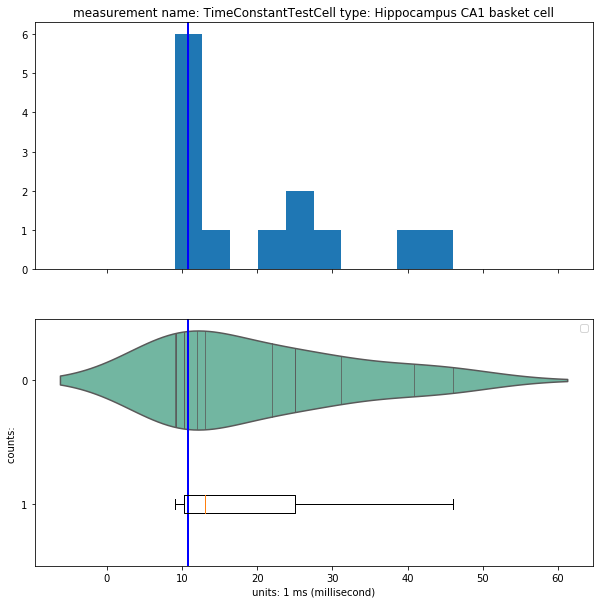
\includegraphics[scale=0.8]{notebooks_converted/needata_thesis_files/needata_thesis_5_7}
%      %\caption{Default model parameterization of the custom written integrator}
%  \label{fig:sub2}
%\end{subfigure}
%
%\caption{Comparison between two Adxaptive Exponential Implementations}
%\label{fig:test}
%\end{center}
%\end{figure}
%
%\end{comment}

%\begin{center}
%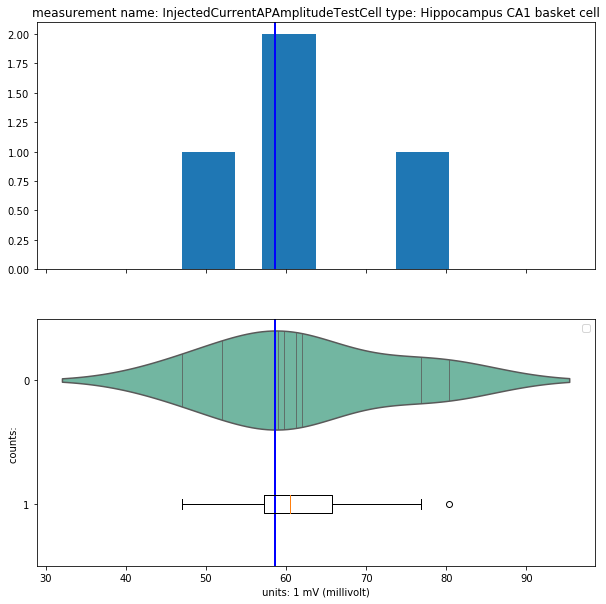
\includegraphics[width=0.7\linewidth]{notebooks_converted/needata_thesis_files/needata_thesis_5_8}
%\end{center}
%
For the majority of cell types and electrophysiological features, the distributions obtained from NeuroElectro were well-described by a normal (or log-normal) distribution.
However, I manually identified and labeled those cases were the data were not so well-behaved, as these might be likely to produced optimized models that did not reflect anything of biological relevance.

Some methods for hypothesis testing that a distribution is unimodal exist \citep{maechler2013package}, however I achieved greater quality control by simply inspecting each case in a peace-meal graphic manner. % manually means to do something by hand. 
I estimated that across all NeuroElectro data sampled here, about $2/3$ is well represented by a unimodal and normal-ish distribution (e.g. Figure \ref{fig:normal-feature} and Figure \ref{fig:normal-feature2}.
In the remaining $1/3$ where this did not hold, I observed a small but still significant number of odd cases: highly skewed distributions (Figure \ref{fig:skewed-feature}), bimodal distributions (Figure \ref{fig:bimodal-feature}), uniform-like distributions (Figure \ref{fig:uniform-feature}), and distribution with insufficient samples to make any judgement at all.

\begin{figure} 
    \begin{center}
   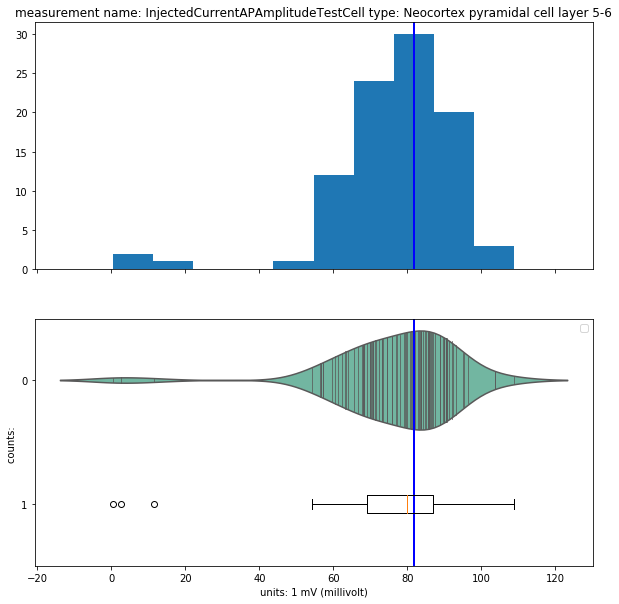
\includegraphics[scale=0.8]{figures/mean_well_served.png}
   \caption[AP Threshold Data Distribution, Layer 5 Pyramidal Cell]{The majority of Neuroelectro data sets were well served by a Gaussian normal distribution. As you can see in this plot the mean is surrounded by a very high density of samples, which slowly thin out with increasing distance from the mean. The distribution is approximately symmetrical, or as symmetrical as one might hope when examining real data sets.}
   \label{fig:normal-feature}
    \end{center}
\end{figure}   

\begin{figure} 
    \begin{center}
    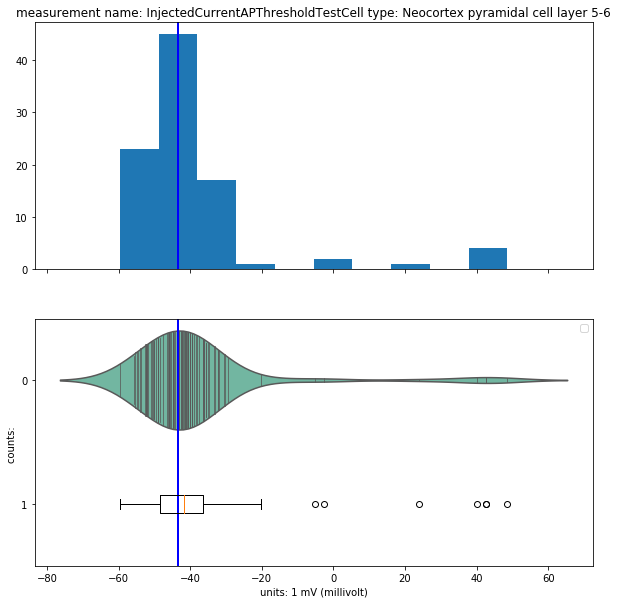
\includegraphics[scale=0.8]{figures/mean_well_served2.png}
    \end{center}
    \caption[AP Amplitude Data Distribution, Layer 5 Pyramidal Cell]{Although the data is skewed to the left and it has outliears. I believe this data distribution is symmetrical enough, to be considered "overall" a normal distribution. In this plot the mean is surrounded by a very high density of samples, which slowly thin out with increasing distance from the mean, although there are a small proportion of outliers these are likely explained by experimental noise.}
    \label{fig:normal-feature2}
\end{figure}   
 
\begin{figure} 
    \begin{center}   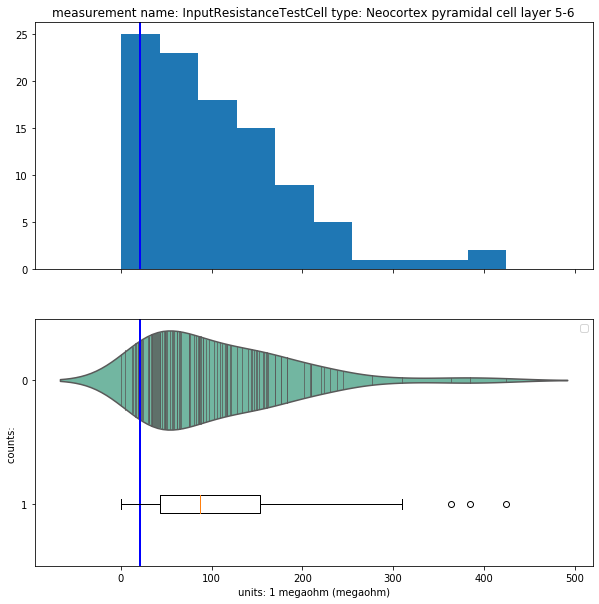
\includegraphics[scale=0.8]{figures/skewed_distribution.png}
    \end{center}
    \caption[Example of skewed NeuroElectro data]{In this distribution of Input Resistance for the Neo-cortical Pyramidal neuron, one can see that values are skewed, and fall off quickly to the right, in this case the median represents the middle of the data better than the mean or the mode.}
    \label{fig:skewed-feature}
\end{figure}   


%\begin{figure} 
%\caption[NeuroElectro data - uniform distribution]{}
%    \begin{center}
%    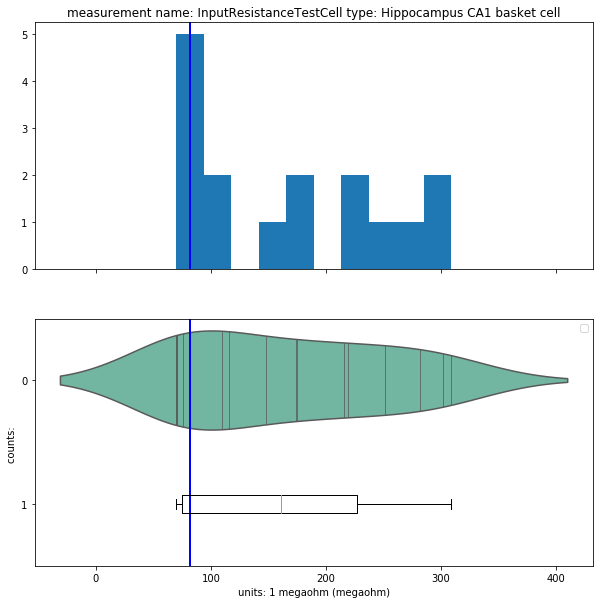
\includegraphics[scale=0.8]{figures/uniform_distribution.png}
%    \end{center}
%\end{figure}       
%%
% Neuronunit code handles under sampled neuroelectro code.
%\begin{figure} 
%\caption[NeuroElectro data - undersampled distribution]{}
%    \begin{center}
%    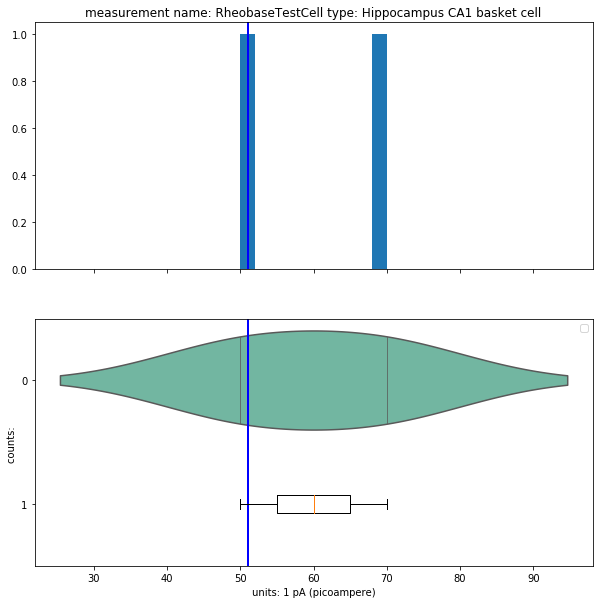
\includegraphics[scale=0.8]{figures/undersampled_distribution.png}
%    \end{center}
%\end{figure}   
%%
    
%\begin{figure} 
%    \begin{center}
%   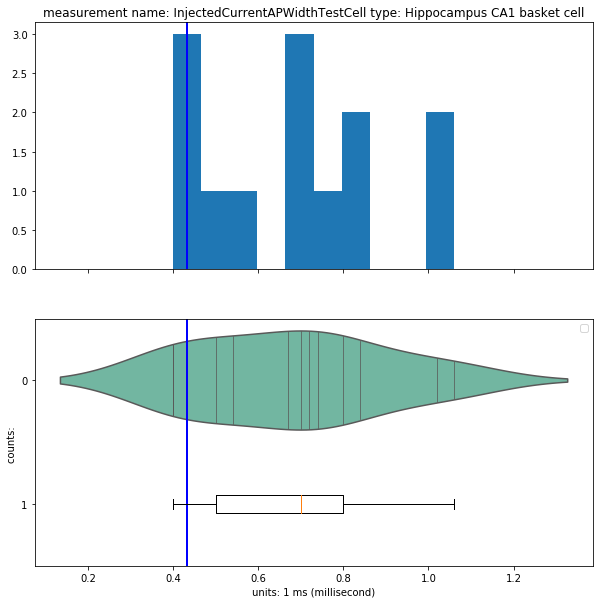
\includegraphics[scale=0.8]{chapters/notebooks_converted/needata_thesis_files/needata_thesis_5_9}
%   \caption{The Action Potential Width of the Hippocampus CA1 basket cell possibly has either an underlying uniform distribution or a multimodal distribution. Since the samples are few, the true distribution is unknown. If the distribution is uniform the gaps in the distribution, that give the histogram a multimodal appearance, as the sample size is lower enough that such gaps may only represent missing samples.}
%    \end{center}
%\end{figure}


%\begin{figure}   
%\begin{center}
%   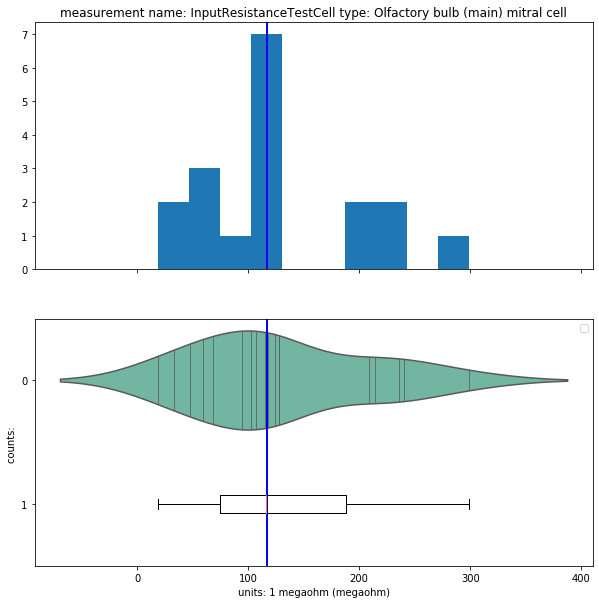
\includegraphics[scale=0.8]{chapters/notebooks_converted/needata_thesis_files/needata_thesis_5_21}
%         \caption[Input Resistance Olfactory Neuron, Perhaps Bimodal]{Input resistance of the Olfactory Mitral cell showed some tendency towards underlying bi-modal distribution, however in the second block of histogram bins, centered around $200-300pA$ only contains approximately $5$ samples. Due to a lack of samples it is also possible to conclude that the data belong to an under sampeled uniform distribution. This data set was important, as one Olfactory neuron test was constructed from this data.}
%\end{center}
%\end{figure}
   
\begin{figure}  
\begin{center}     
  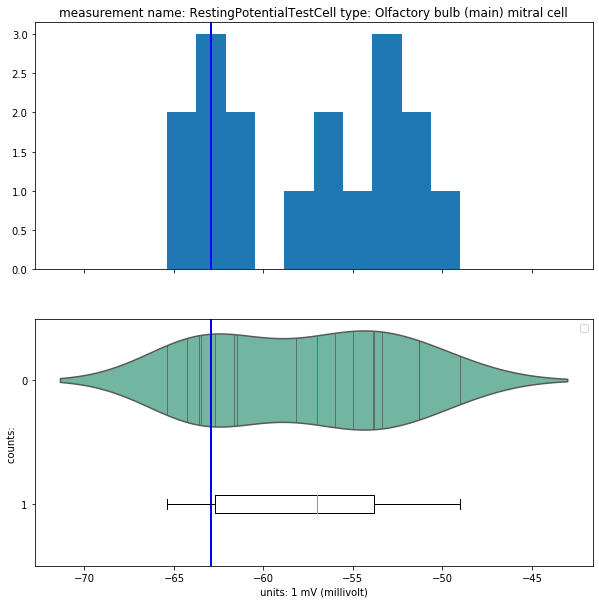
\includegraphics[scale=0.8]{chapters/notebooks_converted/needata_thesis_files/needata_thesis_5_22}
      \caption{Among different measurement sources of neuroelectro data, the resting membrane potential of the Olfactory Mitral cell, showed the greatest tendency of an underlying bi-modal distribution
      In the top panel of this plot we see a binned histogram of Resting membrane potential in the olfactory mitral cell. Although excluded here for considerations of brevity, the input resistance of the olfactory neuron, also perhaps followed a bi-modal or uniform distribution. 
      }
      \label{fig:bimodal-feature}
\end{center}     
\end{figure}
%%
% There are plenty of examples of bi-modal distributions in measurements from cells which are not relevant to this work.
%
%\begin{figure}
%  \centering
%  \includegraphics[scale=0.8]{chapters/notebooks_conv%erted/needata_thesis_files/needata_thesis_5_6}
%   \caption{Default model parameterization of the custom written integrator}
%  \label{fig:sub2}
%\end{figure}
%\begin{figure}
%\begin{center}
%includegraphics{chapters/notebooks_converted/needata_thesis_files/needata_thesis_5_13}
%\end{center}
%\end{figure}
    
\begin{figure}
\begin{center}
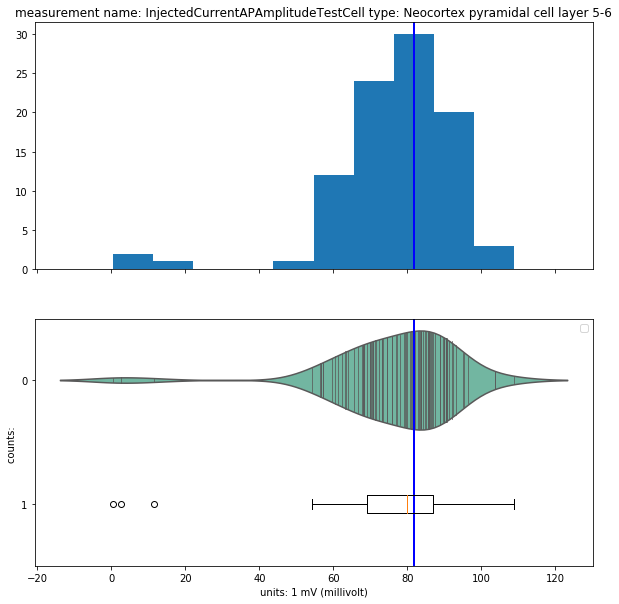
\includegraphics[width=0.7\linewidth]{chapters/notebooks_converted/needata_thesis_files/needata_thesis_5_16}
\caption{This is a binned histogram of Neuroelectro spike width measurements in the Neocortical Pyramidal neuron.
The mode is of the distribution is denoted by a blue vertical line. In this way the mode of the data distribution can be compared to the mean in the box plot. Often modes, and means of the measurements disagree, as they do in the case of CA1 basket cell spike widths. When consulting NeuroElectro measurement, a very common distribution shape is one which is possibly uniform, or multi-modal. It is perhaps obvious but worth noting that a uniform distribution, is not well described by a normal distribution. Under a normal distribution a range of measurement values are equally likely to occur.}
\label{fig:uniform-feature}
\end{center}
\end{figure}

\begin{figure}
\begin{center}
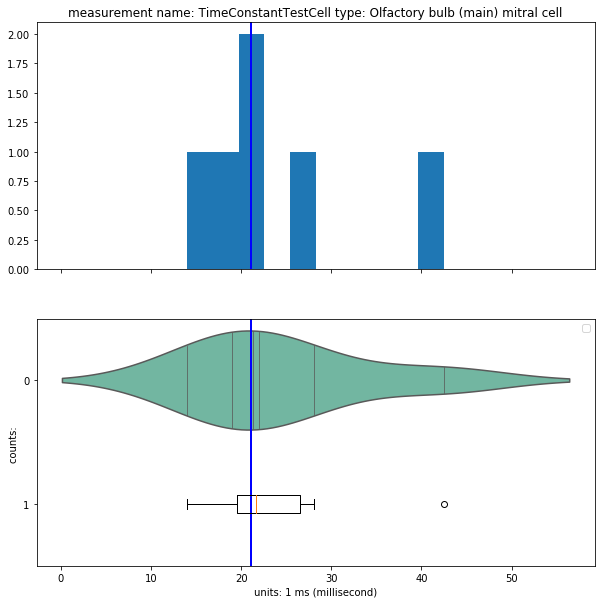
\includegraphics[scale=0.8]{chapters/notebooks_converted/needata_thesis_files/needata_thesis_5_23}
\caption{Similar to the figure above, but for a different neuron type.}
\label{fig:uniform-feature2}
\end{center}
\end{figure}

\subsection{EFEL and The Allen Institute Cell Types Database}
The Blue Brain Project developed the Electrophysiology Feature Extraction Library (EFEL) \citep{EFEL}. Although EFEL computes common spike train statistics related to spike timing, approximately 2/3rds of features extracted by EFEL pertain to spike shapes, and some of those features are shown below. The Allen SDK comes with a very comprehensive python based feature extraction suite. Just like EFEL, the Allen suite does well to represent a large number of spike shape measurements as well as spike train statistics. Unfortunately, the Allen SDK feature extractor is significantly slower than EFEL as EFEL was implemented using the very fast language $C++$. The performance cost may not be felt when dispatching single runs, but slow performance is a significant impediment to optimization. In optimisation feature extraction is directly coupled to chromosome fitness calculations, and it is executed very often across the evolution of the genetic algorithm. Additionally by default, the AllenSDK feature extractor assumes that its user will be applying very high sample frequency and noisy NeuronData Without Borders \citep{teeters2015neurodata} encoded traces. These traces require filtering before they can have Allen features computed on them. Significant intervention is required to turn off filtering. In appropriately applying filtering to model traces causes problems, because the the lower sampling frequency intrinsic to simulated model traces is not predicted by the digital filter. Overall, the EFEL was fast enough to be useful, and its default settings where appropriate to my use case. 
% Membrane potential waveforms where already stored in a container Neo Neo 
\cite{garcia2014neo}


The data available through NeuroElectro covers a large number of cell types, but recording conditions and measurement algorithms are heterogeneous.
It is unclear if the distribution of measurements across such an ensemble is actually a good summary of any one, real cell.
In order to ensure that reduced models could be optimized against data recorded exclusively from single neurons, I also used the Allen Institute Cell Types Database \citep{celltypes}, a project of the Allen Institute for Brain Science.
This Cell Types database consists of summary physiological, morphological, and histological data for thousands of individual neurons (across a few dozen subtypes) from mouse visual cortex, obtained using patch clamp recordings in slices.
Each experiment is done using exactly the same methods and with the same sequence of stimuli (described in \cite{celltypes}), ensuring not only that models generated using this data are directly comparable, but that each such model is reflective of a single neuron.

The Cell Types Database does provide some limited pre-computed measures of action potential waveform details. 
However, the data is not organized in a way that makes it is useful for the types of optimization and data analysis I perform here.
Specifically, I require features that are computed on cell responses to current injection values that are fixed multiples of rheobase.
Additionally, the pre-computed features are thin relative to those that I brought to bear in the optimizations described in the Results section.
Because raw data is available through the Cell Types API, I therefore re-computed all necessary features from this raw data, according to the consistent standard reflected in the NeuronUnit code.

In contrast to NeuroElectro, the Cell Types database also has a great deal more information relevant to the above threshold dynamics of neurons, such as the number and pattern of action potentials they discharge in response to somatically-injected currents much larger than rheobase, or in response to non-square injected currents.
In order to exploit these, I developed several additional NeuronUnit tests using EFEL, such as: ``time to first spike test" and ``mean AP amplitude test". In principal any feature measured in the Cell Types Data could be upgraded to a NeuronUnit test, and I created a code-generation template to accelerate this task.
I also created some tests from scratch, especially those adapted from other descriptions of feature extraction from the literature (as described in sections \ref{sec:allensdk}, \ref{sec:efel}, and \ref{sec:elephant}. These are shown in Table \ref{tab:featurez}.


\begin{table}
\centering

\resizebox{\textwidth}{!}{
\begin{tabular}{ll}
            \textbf{Test Name} & \textbf{Test Description}\\
adaptation-index & Measures spiking fatigue in response to constant current\\
 adaptation-index2 & The same as Adaption index1, except it is used as an alternative when spikes below $0mV$ occur.   \\
time-to-first-spike & amount of time elapsed until first spike \\ mean-AP-amplitude & The average spike height in a spike train \\
spike-half-width & The width of a spike is obtained at point when spike height is half its total amplitude\\    
AHP-depth & The after hyperpolarisation depth\\
minimum-voltage & The minimum voltage\\
peak-voltage & the maximum voltage, usually a spike peak. \\
time-to-last-spike & The time of last spike onset \\
AHP-depth-abs & After Hyperpolarisation depth.\\
all-ISI-values & All interspike interval times\\
voltage-base & minimum voltage while undergoing stimulus, often below the threshold of APs. \\
min-voltage-between-spikes & Needed because during  high frequency firing AHPs may be skipped.\\
Spikecount & Just the number of spikes that occured in the provided stimulus window\\
\end{tabular}}
\caption[List of features]{A number of features that were encoded into NeuronUnit tests for optimization}
\label{tab:features}
\end{table}

Below I include some graphs of the many different features utilized in optimization.

\begin{figure}
    \centering
    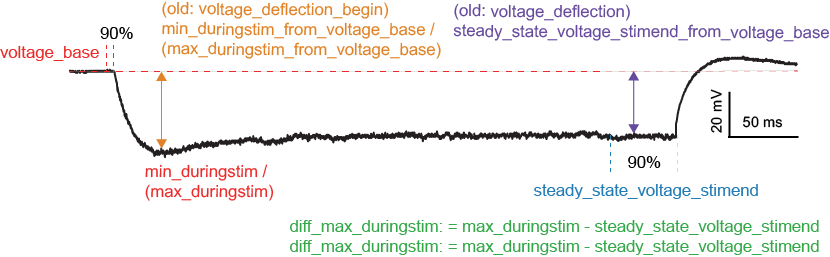
\includegraphics{figures/voltage_features.png}
    \caption[Passive membrane properties probed with a negative amplitude current stimulus]{Although applying a negative current stimulus, only tends to activate so called ``passive" ion channels in the membrane, probing the neuron membrane in this way is simple way of ascertaining essential information about neuron membrane resistance and capacitance. Figure taken from \url{https://efel.readthedocs.io/en/latest/eFeatures.html}}
    \label{fig:voltage_figures}
\end{figure}

\begin{figure}
    \centering
    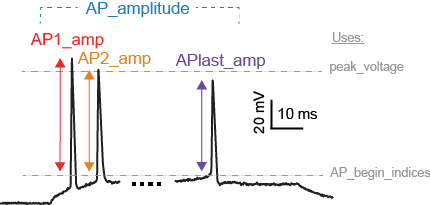
\includegraphics{figures/AP_Amplitude.png}
    \caption[]{When a neuron fires multiple spikes, many features in the waveform are readily measurable, these include, mean AP overshoot, every AP amplitude, wave troughs, spike threshold and after hyperpolarisation potential to name a few}
    \label{fig:features_example}
\end{figure}

\begin{figure}
    \centering
    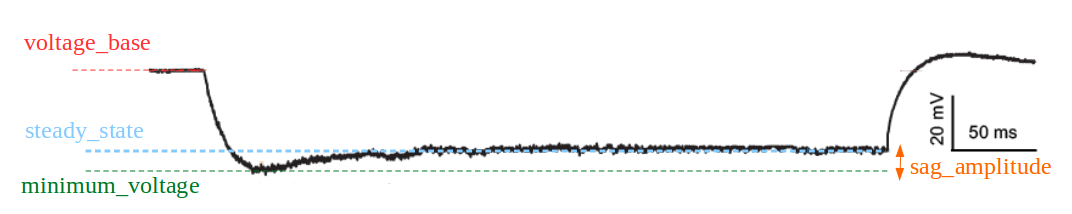
\includegraphics{figures/sag_amplitude}
    \caption{Caption}
    \label{fig:sag_amplitude}
\end{figure}

%XXXX Russell, can you list the new tests above.

These tests can be used to assess the agreement between model and biological neurons on suprathreshold dynamics, largely reflected in patterns of spiking such as bursting and adaptation, but also mean spike height, and mean spike width

\subsection{The Blue Brain Project Neocortical Microcircuit Portal}
\label{sec:bluebrain-data}
I also made use of one additional data source, the The Blue Brain Project Neocortical Microcircuit Portal, similar in some ways to the Allen Institute Cell Types Database but reflecting measurements taken from mouse somatosensory cortex (again in patch-clamp recordings from slices).
From this dataset I exclusively used a collection of experiments from animal B-95, which for reasons unknown yielded a tremendous amount of data (\url{http://microcircuits.epfl.ch/#/animal/8ecde7d1-b2d2-11e4-b949-6003088da632}).
Conceptually, this dataset added anything new, but it did allow for high-quality optimized models to be produced from another brain region (somatosensory, rather than visual cortex).
These data are also linked to--and constrain--the on-going Human Brain Project effort to simulated biophysically-detailed multi-compartmental models of the same neurons (and whole neural circuits).
This means that the reduced models produced here can be compared directly to those more detailed models, or that the general NeuronUnit-driven genetic optimization framework developed here could be used to optimize detailed models which should, in principle, be similar to those produced through the larger Human Brain Project effort.
Indeed, the Human Brain Project is already a user of the SciUnit framework developed in my lab, on which NeuronUnit is based.

The tests which lead to the best fits in the above threshold experiments, where the tests derived from the above EFEL features applied to NeuronUnit data (Figure \ref{fig:supra-threshold-tests}), the measurement type, and the test type did not change between Allen Cell Types, and Blue Brain Data, only the reference data which informed comparison measurements changed.

The table below is constitutes a summary of both NeuroElectro and Allen experimental data reports. This data can naturally be reported in tabular form. 

\subsection{The Experimental Measurements}

\begin{table}[ht]
\centering
\resizebox{\textwidth}{!}{
\begin{tabular}{lllllllll}
\toprule
name & Hippocampus CA1 pyramidal cell & Cerebellum Purkinje cell & Neocortex pyramidal cell layer 5-6 &      olf\_mit &      623960880 &      623893177 &      471819401 &      482493761 \\
\midrule
RheobaseTest                   &                      189.24 pA &                680.79 pA &                          213.85 pA &          NaN &        70.0 pA &       190.0 pA &       190.0 pA &        70.0 pA \\
InputResistanceTest            &                    107.08 Mohm &              142.06 Mohm &                        120.67 Mohm &  130.08 Mohm &  241.0 megaohm &  136.0 megaohm &  132.0 megaohm &  132.0 megaohm \\
TimeConstantTest               &                        24.5 ms &                      NaN &                           15.73 ms &     24.48 ms &        23.8 ms &        27.8 ms &        13.8 ms &        24.4 ms \\
CapacitanceTest                &                        89.8 pF &                620.27 pF &                          150.58 pF &    235.75 pF &            NaN &            NaN &            NaN &            NaN \\
RestingPotentialTest           &                      -65.23 mV &                -61.59 mV &                          -68.25 mV &    -58.14 mV &       -65.1 mV &       -77.0 mV &       -77.5 mV &       -71.6 mV \\
InjectedCurrentAPWidthTest     &                        1.32 ms &                  0.41 ms &                            1.21 ms &      1.61 ms &            NaN &            NaN &            NaN &            NaN \\
InjectedCurrentAPAmplitudeTest &                       86.36 mV &                 71.23 mV &                           80.44 mV &      68.4 mV &            NaN &            NaN &            NaN &            NaN \\
InjectedCurrentAPThresholdTest &                       -47.6 mV &                -46.89 mV &                          -42.74 mV &     -38.9 mV &            NaN &            NaN &            NaN &            NaN \\
FITest                         &                            NaN &                      NaN &                         0.05 Hz/pA &          NaN &     0.18 Hz/pA &     0.12 Hz/pA &     0.18 Hz/pA &     0.09 Hz/pA \\
\bottomrule
\end{tabular}}
\end{table}

